\section{Milan --- Ecopass and Area C}\label{sec:milan}

\subsection{Implementation}

To frame the the Milan experience requires two pieces of context.\footnote{This history is based on \citet{Mattioli2012}, with support from \citep{Rotaris2010}.} First, Italian cities commonly operate ``limited traffic zones'' (ZTL's), areas where vehicle access is restricted. A ZTL, for instance, might ban private vehicles during the workday except for residents. Milan already had a camera-enforced ZTL inside its Cherchia dei Bastioni (CB)---a ring of 16th century fortifications around the city center where about 80,000 people live---so charging required little new infrastructure. Second, Milan has relatively high use of cars and motorcycles---especially those with diesel engines---and is located in the relatively windless Po Valley. The combination of geography and vehicle use has begotten severe particulate matter pollution, leading to constant violation of European Union directives on air quality. Thus, while other cities have touted their schemes' environmental impacts, Milan is the only city which has explicitly designed a DCP scheme to combat air pollution.

 Letizia Moratti proposed charging for access to the CB following her election as Mayor of Milan in 2006. On January 1, 2008 launch of ``Ecopass,'' an ANPR-enforced daily license (one charge pays for unlimited travel). Ecopass had a complex charging structure (see Table \ref{tab:milan-ecopass-prices}) and liberal exemptions---especially green vehicles. Thus, the share of chargeable vehicles entering the zone fell sharply in the first few years. Observers believed Ecopass was not having its advertised effect, particularly since air pollution worsed in early 2010. Consequently, in 2010 activists organized a petition drive for a number of environmental and transportation referenda, including one to extend road pricing to all cars and to extend the charging area. In the July 2011 referendum, all the proposed measures passwed, including the Ecopass proposal with 79 percent of votes cast. Around the same time, Moratti was replaced as mayor by Giuliano Pisapia, who set about remaking Ecopass. The reorganized system, rebranded ``Area C,'' commenced operation on January 16, 2012. Area C does not have a larger charging zone, but it does charge more vehicles.

\subsection{Design}

The charging zone of both Area C and Ecopass is an 8 km$^{2}$ area of central Milan called the Cerchia dei Bastioni (CB) (see Figure \ref{fig:milan-map}). The cordon consists of 43 access points where cameras read the number plates of vehicles entering (but not exiting). Like the LCC, charges are flat over the day; they are in force from 7:30 AM to 7:30 PM on weekdays, except that since September 2012 Area C stops charging at 6 PM on Thursdays in order to promote a night of shopping and cultural events \citep{CorriereDellaSera2012}. 

The standard way to pay is to buy a digital ``ticket'' at banks, parking meters, online, ATM's or in stores and then ``activate it''---that is, associate it with a plate number on a particular day---by phone, SMS, online or at municipal offices. One has until midnight until the day after entry to pay, although it is also possible to pay in advance. Since the switch to Area C, users can also sign up for a Telepass radio-frequency transponder to pay by debit automatically. 

What most distinguishes Ecopass from Area C is the charging structure: Ecopass involved a schedule of five emission classes, while Area C involves three user classes: resident, ``service vehicle'' and standard. See Tables \ref{tab:milan-ecopass-prices} and \ref{tab:milan-area-c-prices}. ``Service'' vehicles are mostly commercial vehicles for delivery and construction, as defined according to complex rules which change over time. 

Both systems have many exemptions and caveats. Motorcycles and scooters, electric vehicles, certain green vehicles, taxis, public buses and certain emergency or government vehicles have been exempt under both schemes. Instead of Ecopass' sliding scale, Area C simply bans most high emission vehicles and vehicles longer than 7.5 meters, with some exceptions, while exempting a changing number of green vehicles. The list of exemptions and prohibitions changes from time to time: for instance, in February 2017 LPG and CNG vehicles lost their exempt status, while certain diesel vehicles were banned. Ecopass offered residents of the CB a 50\% discount on their first 50 entries per year and a 40\% discount on the next fifty; but under Area C residents receive 40 free days per year and thereafter pay the \euro 2 residents rate. Since late 2012, the standard charge is only \euro3 for vehicles which park for four or more hours at a garage participating in an agreement with the city government. Finally, Ecopass lets certain licensed buses for tourists and students that longer than 7.5m can enter the CB subject to a scale that slides up to \euro 100 with the size of the vehicle.

\begin{figure}[ht]
	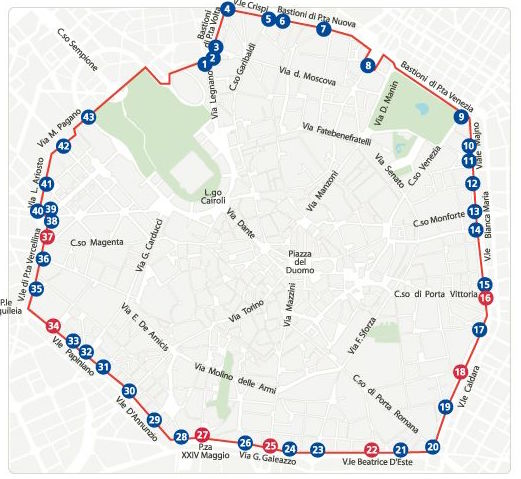
\includegraphics[width=.8\textwidth]{../img/milan-map.jpg}
	\caption{Milan Ecopass/Area C \citep{Rotaris2010}}
	\label{fig:milan-map}
\end{figure}

\begin{table}
\begin{center}
\begin{tabular}{|>{\centering}m{1.8cm}|>{\centering}m{1.8cm}|>{\centering}p{1.8cm}|}
\hline 
Emissions Class & Charge (\euro) \tabularnewline
\hline 
\hline 
1 & 0 \tabularnewline
\hline 
2 & 0 \tabularnewline
\hline 
3 & 2 \tabularnewline
\hline 
4 & 5 \tabularnewline
\hline 
5 & 10 \tabularnewline
\hline 
\end{tabular}
\par\end{center}
\caption{Ecopass prices. Lower classes are less polluting. Class I includes hybrid and electric cars. Class V low-efficiency diesel and buses. \citep{Rotaris2010} }\label{tab:milan-ecopass-prices}
\end{table}

\begin{table}

\begin{center}
\begin{tabular}{|>{\centering}m{2.2cm}|>{\centering}m{1.8cm}|}
\hline 
User Class & Charge (\euro)\tabularnewline
\hline 
\hline 
standard & 5\tabularnewline
\hline 
residents & 2\tabularnewline
\hline 
service vehicle & 3\tabularnewline
\hline 
\end{tabular}
\par\end{center}
\caption{Area C prices. ``Service vehicles'' are those enaged in certain commercial activities.}\label{tab:milan-area-c-prices}
\end{table}

\subsection{Transportation impacts}

Milan has the smallest literature of any of the schemes we visit. Still, the city has collected a great deal of data on traffic flow and emissions and has published annual reports on both Ecopass and Area C's impacts.\footnote{http://www.comune.milano.it/wps/portal/ist/it/servizi/mobilita/Area\_C/motivazioni}  

In the first year of Ecopass, entries to the CB during charging hours fell 14.6\% \citep[Tab. 2, p. 145]{Croci2015}. From 2008 to 2011, traffic recomposed quickly: in 2008, 22\% of entering vehicles paid the toll, but by 2011 the share had fallen to 14.1\%. See Fig. XXX for the trend of paying vs exempt traffic from Jan. 2008 to June 2010. The number of vehicles in the most polluting classes (classes 3-5 of Tab. \ref{tab:milan-ecopass-prices}) fell 70\%.

The switch to Area C coincided with a further reduction in entries which has been sustained (see Fig. \ref{fig:milan-entries}). The charged share has risen substantially: in 2016, 56\% of vehicles are subject to charge---four times the 14.1\% observed under Ecopass \citep[p. 13]{AMAT2017}.

Comparisons of private vehicle speeds seem only to be reported for the first year of Ecopass, when speed in the CB rose 4\% during the morning rush \citep{AMMA2009}. Public transit speeds increased more, but this effect was probably due to new bus lanes.

\begin{figure}[ht]
	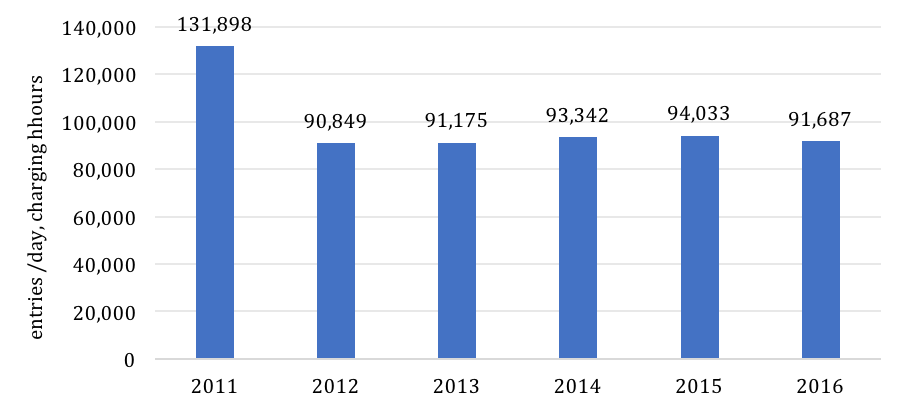
\includegraphics[width=\textwidth]{../img/milan-entries2.png}
	\caption{Entries to the Cerchia dei Bastioni. 2011 was the last year of Ecopass; years following are under Area C. \citep[p. 9]{AMAT2017}}
	\label{fig:milan-entries}
\end{figure}

In 2012, protests by owners of parking garages in the CB led to a court-ordered suspension of charging that lasted from from 25 July to September 17; because of its random nature, have used the suspension as an experiment to test the scheme's effects. \citet{Gibson2015} reaches conclusions regarding the effect of Area C on entries and pollution very different from \citet{Percoco2013} and \citet{Percoco2014}, and the studies even seem to have different data. But all three studies agree that Area C encourages the use of motorcycles, which are exempt---a finding that \citet{Percoco2013} says greatly reduces Area C's power to curb pollution.

\subsection{Finances}

\citet{Rotaris2010} say that implementation costs for Ecopass are not available, but were not very high, since Area C used the same infrastructure as the existing ZTL. Operating costs were \euro 6.5M in 2008 \citep[p. 49]{AMMA2009}. Ecopass revenues were \euro 12.6M in 2008 (the first year), but traffic recomposed toward less-taxed or exempt vehicles, and so revenue fell to \euro 9.6M by 2009 \citep[p. 51]{AMAT2010}. 

Area C has proven more profitable. In 2012, Area C earned \euro 20M and cost \euro 7M to operate \citep{Beria2015}. It does not seem that there were implementation costs for switching to Area C.\footnote{\citet{Croci2016} cites operating costs of \euro 14M and implementation costs of Area C, but the source they provide is a URL on the City of Milan website that is now non-functioning, and this seems to contradict other sources from the City of Milan.} Of the \euro 13 M profit, \euro 3 M went to the BikeMi bikeshare program and \euro 10M to public transport. Area C made \euro 28.3M in 2015 \citep[p. 28]{Milan2016} and \euro 32.3 M in 2016 \citep[p. 25]{Milan2017}, but these figures only count toll revenue---not penalties. 

Penalties for non-compliance seem to have been an major source of revenues. No official data on fines are available, but \citet{Rotaris2010} cites informal sources claiming  penalties for Ecopass exceeded tolls. This estimate seems reasonable in light of the fact that, from 2012-2014 (inclusive), Area C earned roughly \euro 60-75 M in penalties, due to unfamiliarity with the system. Penalties declined each of those years, but in February 2017, Area C was altered such that many alternative fuel cars (e.g., LPG and CNG) lost their exemption and several types of diesel vehicle were banned from the charging zone, leading to a surge in penalties as drivers struggled to adapt.

